%=================================================================
\DIFdelbegin %DIFDELCMD < 

%DIFDELCMD < %%%
\DIFdelend \section{Introduction}\label{sec-intro}


%\todo{Narrow down to a topic; Dig a hole; Fill the hole}
\DIFaddbegin \todo{Formula for Introduction}
\DIFaddend 



%\gangli{``narrow in on topic'' reminds you 
%that readers and reviewers only know that this is a AI or HTM research paper (and maybe have read the title/abstract). 
%You need to help them figure out what topic and area of research paper this is. 
%You _don't_ need to wax poetic about the topic's importance.}

%\gangli{`dig a hole'' reminds you that 
%you need to convince the reader that there's a problem with the state of the world. 
%Prior work may exist but it's either missing something important or there's a missing opportunity. 
%The reader should be drooling for a bright future just out of reach.}

%\gangli{``fill the hole'' reminds you to show the reader 
%how and why the paper they're reading will fix these problems and deliver us into a better place. 
%You don't need a whirlwind summary of the technical details, 
%but you need readers convinced (and in a good mood) to keep reading.}

\DIFaddbegin \gangli{A good paper introduction is fairly formulaic. 
If you follow a simple set of rules, 
you can write a very good introduction. 
The following outline can be varied. 
For example, 
you can use two paragraphs instead of one, 
or you can place more emphasis on one aspect of the intro than another. 
But in all cases, 
all of the points below need to be covered in an introduction, 
and in most papers, 
you don't need to cover anything more in an introduction.}



\DIFaddend %\todo{The importance of the area}
%\blindtext
\DIFaddbegin \todo{Motivation}
\DIFadd{At a high level, 
what is the problem area you are working in and why is it important? 
It is important to set the larger context here. 
Why is the problem of interest and importance to the larger community?
}\DIFaddend 


\DIFdelbegin \DIFdel{Sales forecasting using time series is one of the most important applications in business and economics. It helps businesses make production plans, inventory management, sales and marketing strategies, etc. based on the predicted future sales. 
Time series forecasting can be done using various models and algorithms such as linear regression, exponential smoothing, ARIMA, neural networks, etc. 
}%DIFDELCMD < 

%DIFDELCMD < %%%
\DIFdelend %\todo{The problems faced by most current methods}
%\blindtext
\DIFdelbegin %DIFDELCMD < 

%DIFDELCMD < %%%
\DIFdel{This sales forecasting task has multiple factors that need to be considered. It is necessary to take into account the impact of multiple factors on the forecasting goal. 
Consider how to perform data analysis to simplify the model prediction goal. 
}\DIFdelend \DIFaddbegin \todo{What is the specific problem considered in this paper?}
\DIFadd{This paragraph narrows down the topic area of the paper. 
In the first paragraph you have established general context and importance. 
Here you establish specific context and background.
}\DIFaddend 

%\todo{What can be addressed by existing methods; Why those problems are challenges to existing methods?}
%\blindtext
\DIFaddbegin \todo{Contribution}
\DIFadd{"In this paper, we show that ...". 
This is the key paragraph in the intro - you summarize, 
in one paragraph, 
what are the main contributions of your paper given the context 
you have established in paragraphs 1 and 2. 
What is the general approach taken? 
Why are the specific results significant? 
This paragraph must be really good. 
}\DIFaddend 

\DIFdelbegin \section{\DIFdel{Data Analysis}} %DIFAUXCMD
\addtocounter{section}{-1}%DIFAUXCMD
%DIFDELCMD < \label{sec-preliminaries}
%DIFDELCMD < %%%
\DIFdel{The data covers six countries: Belgium, France, Germany, Italy, Poland, Spain, two stores: KaggleMart, KaggleRama, and four products.The training set timeline is from 2017 to 2020, and the test set timeline is 2021.
Firstly, the monthly sales volume of the overall data is analyzed.This paper finds that there is a cyclical trend in the change of sales.
}\DIFdelend \DIFaddbegin \DIFadd{You should think about how to structure these one or 
two paragraph summaries of what your paper is all about. 
If there are two or three main results, 
then you might consider itemizing them with bullets or in test. 
}\begin{itemize}
	\item \DIFadd{e.g., First ...
	}\item \DIFadd{e.g., Second ...
	}\item \DIFadd{e.g., Third ...
}\end{itemize}
\DIFadd{If the results fall broadly into two categories, 
you can bring out that distinction here. 
For example, "Our results are both theoretical and applied in nature. 
(two sentences follow, one each on theory and application)"
}\DIFaddend 

\DIFdelbegin %DIFDELCMD < \begin{figure}[!h]
%DIFDELCMD < 		\centering
%DIFDELCMD < 		\selectcolormodel{rgb}
%DIFDELCMD < 		\includegraphics[scale=0.23]{month.eps}
%DIFDELCMD < 		%%%
%DIF <   \includegraphics[width=0.5\textwidth]{figures//OutAspect_target.eps}\\
		%DIFDELCMD < \caption{%
{%DIFAUXCMD
\DIFdelFL{Monthly sales}}%DIFAUXCMD
%DIFDELCMD < \label{fig:OutAspect-target}
%DIFDELCMD < \end{figure}
%DIFDELCMD < %%%
\DIFdel{Analysis of the store factors will be conducted next. By calculating the daily sales ratio of each store, 
it is found that KaggleMart's sales ratio remains around 75\%, 
while KaggleRama's sales ratio is 25\%. This indicates that the sales ratio of stores is almost fixed and unchanged.
}\DIFdelend %DIF > \todo{What provides the motivation of this work? What are the research issues? What is the rationale of this work? }
%DIF > \blindtext
\DIFaddbegin \todo{At a high level what are the differences in what you are doing, and what others have done? }
\DIFadd{Keep this at a high level, 
you can refer to a future section where specific details and differences will be given. 
But it is important for the reader to know at a high level, 
what is new about this work compared to other work in the area.
}\DIFaddend 

\DIFdelbegin %DIFDELCMD < \begin{figure}[H]
%DIFDELCMD < 	\centering
%DIFDELCMD < 	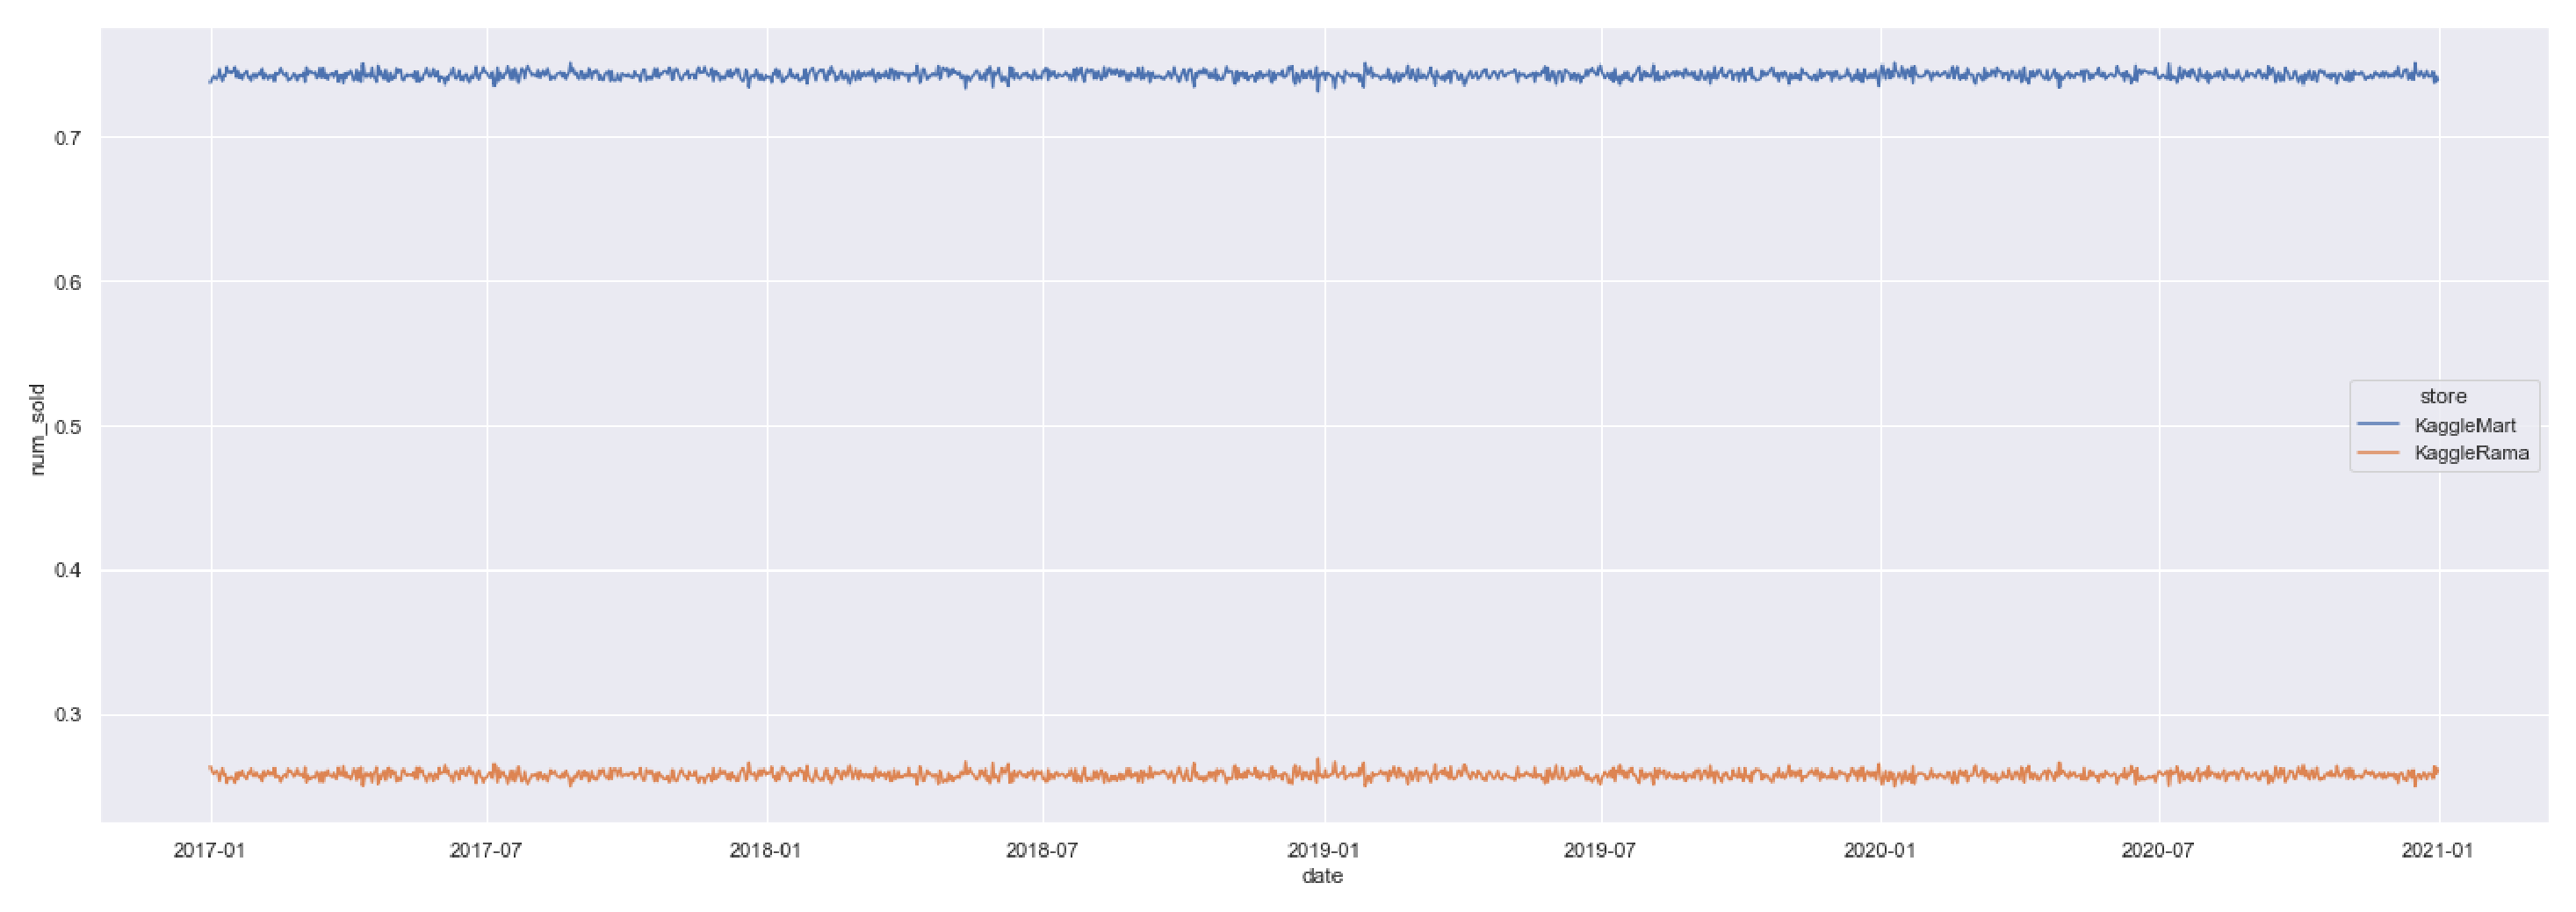
\includegraphics[scale=0.21]{store-ratio.eps}
%DIFDELCMD < 	%%%
%DIF <   \includegraphics[width=0.5\textwidth]{figures//OutAspect_target.eps}\\
	%DIFDELCMD < \caption{%
{%DIFAUXCMD
\DIFdelFL{Stores ratio}}%DIFAUXCMD
%DIFDELCMD < \label{fig:OutAspect-target}
%DIFDELCMD < \end{figure}
%DIFDELCMD < 

%DIFDELCMD < %%%
\DIFdel{For more intuitive performance, this paper takes the sales volume of KaggleMart as the benchmark, and multiplies the sales volume of KaggleRama by a weight value to remove the impact of the ratio. The observation chart shows that their sales volume change curves almost coincide, indicating that their sales volume is only related to the total sales volume and has nothing to do with the factors of the store itself}\DIFdelend %DIF > \todo{What we have done and what are the contributions.}
%DIF > \blindtext
\DIFaddbegin \todo{A roadmap for the rest of the paper}
\DIFadd{"The remainder of this paper is structured as follows..." 
Give the reader a roadmap for the rest of the paper. 
Avoid redundant phrasing, 
"In Section 2, In section 3, .}\DIFaddend .\DIFaddbegin \DIFadd{. In Section 4, ... " etc.
}\DIFaddend 

\DIFdelbegin %DIFDELCMD < \begin{figure}[htb]
%DIFDELCMD < 	\centering
%DIFDELCMD < 	\selectcolormodel{rgb}
%DIFDELCMD < 	\includegraphics[scale=0.225]{store-trend.eps}
%DIFDELCMD < 	%%%
%DIF <   \includegraphics[width=0.5\textwidth]{figures//OutAspect_target.eps}\\
	%DIFDELCMD < \caption{%
{%DIFAUXCMD
\DIFdelFL{Stores ratio trend}}%DIFAUXCMD
%DIFDELCMD < \label{fig:OutAspect-target}
%DIFDELCMD < \end{figure}
%DIFDELCMD < %%%
\DIFdel{We analyzed the national factors in the same way and found similar phenomena. The sales volume of each country is different before 2020, 
and the proportion is almost fixed, while the proportion of six countries is the same in 2020. It can also exclude the influence of the country itself and predict the sales volume of each country through the total sales volume. 
}\DIFdelend \DIFaddbegin \gangli{A few general tips:
Don't spend a lot of time into the introduction 
telling the reader about what you don't do in the paper. 
Be clear about what you do do.
Does each paragraph have a theme sentence that sets the stage for the entire paragraph? Are the sentences and topics in the paragraph all related to each other?}
\DIFaddend 

\DIFdelbegin %DIFDELCMD < \begin{figure}[h]
%DIFDELCMD < 	\centering
%DIFDELCMD < 	\selectcolormodel{rgb}
%DIFDELCMD < 	\includegraphics[scale=0.215]{Country-ratio.eps}
%DIFDELCMD < 	%%%
%DIF <   \includegraphics[width=0.5\textwidth]{figures//OutAspect_target.eps}\\
	%DIFDELCMD < \caption{%
{%DIFAUXCMD
\DIFdelFL{Countries ratio}}%DIFAUXCMD
%DIFDELCMD < \label{fig:OutAspect-target}
%DIFDELCMD < \end{figure}
%DIFDELCMD < \begin{figure}[h]
%DIFDELCMD < 	\centering
%DIFDELCMD < 	\selectcolormodel{rgb}
%DIFDELCMD < 	\includegraphics[scale=0.235]{Country-trend.eps}
%DIFDELCMD < 	%%%
%DIF <   \includegraphics[width=0.5\textwidth]{figures//OutAspect_target.eps}\\
	%DIFDELCMD < \caption{%
{%DIFAUXCMD
\DIFdelFL{Countries ratio trend}}%DIFAUXCMD
%DIFDELCMD < \label{fig:OutAspect-target}
%DIFDELCMD < \end{figure}
%DIFDELCMD < %%%
\DIFdelend \DIFaddbegin \gangli{Does each paragraph have a theme 
sentence that sets the stage for the entire paragraph? 
Are the sentences and topics in the paragraph all related to each other?}
\DIFaddend 

\DIFdelbegin \DIFdel{Finally, we will analyze the store and the country together, and use the KaggleMart of Belgium as the benchmark to draw the broken line chart of the flower removal rate.It was found that the sales curve almost coincided.}\DIFdelend \DIFaddbegin \gangli{Do all of your tenses match up in a paragraph?}
\DIFaddend 

\DIFdelbegin %DIFDELCMD < \begin{figure}[H]
%DIFDELCMD < 	\centering
%DIFDELCMD < 	\selectcolormodel{rgb}
%DIFDELCMD < 	\includegraphics[scale=0.23]{Countryandstore-trend.eps}
%DIFDELCMD < 	%%%
%DIF <   \includegraphics[width=0.5\textwidth]{figures//OutAspect_target.eps}\\
	%DIFDELCMD < \caption{%
{%DIFAUXCMD
\DIFdelFL{Countries and Store trend}}%DIFAUXCMD
%DIFDELCMD < \label{fig:OutAspect-target}
%DIFDELCMD < 	\end{figure}
%DIFDELCMD < %%%
\DIFdelend \DIFaddbegin \DIFadd{Test citation~\cite{BL12J01}. 
}\begin{JournalOnly}
\DIFadd{and~\citep{BJL11J01} or~\citet{BJL11J01}.
}\end{JournalOnly}
\DIFaddend 

\DIFdelbegin \DIFdel{After that, we analyzed the change of the proportion of the four commodities and found that there was a two-year cycle of change.}\DIFdelend \DIFaddbegin \DIFadd{This is for~}\cref{tbl:overall-experiments}\DIFadd{, 
}\todo[fancyline]{Testing.}
\DIFadd{and this is for~}\cref{sec-conclusions}\DIFadd{.
}\todo[noline]{A note with no line back to the text.}%DIF > 
\gangli{This is comment from Gang.}
\qwu{Response from QW}
\DIFaddend 

\DIFdelbegin %DIFDELCMD < \begin{figure}[H]
%DIFDELCMD < 	\centering
%DIFDELCMD < 	\selectcolormodel{rgb}
%DIFDELCMD < 	\includegraphics[scale=0.3]{product-trend.eps}
%DIFDELCMD < 	%%%
%DIF <   \includegraphics[width=0.5\textwidth]{figures//OutAspect_target.eps}\\
	%DIFDELCMD < \caption{%
{%DIFAUXCMD
\DIFdelFL{Product ratio trend}}%DIFAUXCMD
%DIFDELCMD < \label{fig:OutAspect-target}
%DIFDELCMD < \end{figure}
%DIFDELCMD < %%%
\DIFdelend \DIFaddbegin \DIFadd{Number:
}\num{123}\DIFadd{.
}\numlist{10;30;50;70}\DIFadd{,
}\numrange{10}{30}\DIFadd{,
}\SIlist{10;30;45}{\metre}\DIFadd{,
and
}\SI{10}{\percent}
\DIFaddend 

\DIFdelbegin \DIFdel{Therefore, we can only predict the total sales volume of each day by aggregating the time series, and then predict the sales volume of various products in stores in various countries by the total sales volume.}\DIFdelend \DIFaddbegin \missingfigure[figcolor=white]{Testing figcolor}
\DIFaddend 


\DIFdelbegin %DIFDELCMD < \begin{figure}[h]
%DIFDELCMD < 	\centering
%DIFDELCMD < 	\selectcolormodel{rgb}
%DIFDELCMD < 	\includegraphics[scale=0.3]{trainline.eps}
%DIFDELCMD < 	%%%
%DIF <   \includegraphics[width=0.5\textwidth]{figures//OutAspect_target.eps}\\
	%DIFDELCMD < \caption{%
{%DIFAUXCMD
\DIFdelFL{Aggregated time series}}%DIFAUXCMD
%DIFDELCMD < \label{fig:OutAspect-target}
%DIFDELCMD < \end{figure}
%DIFDELCMD < %%%
\DIFdelend \DIFaddbegin \begin{ConferenceOnly}
\DIFadd{We have }\SI{10}{\hertz}\DIFadd{,
}\si{\kilogram\metre\per\second}\DIFadd{,
the range: }\SIrange{10}{100}{\hertz}\DIFadd{.
$\nicefrac[]{1}{2}$.
}\DIFaddend 

\DIFdelbegin \section{\DIFdel{Feature Extraction}} %DIFAUXCMD
\addtocounter{section}{-1}%DIFAUXCMD
%DIFDELCMD < \label{sec-method}
%DIFDELCMD < %%%
\DIFdelend \DIFaddbegin \missingfigure{Make a sketch of the structure of a trebuchet.}
\DIFaddend 

\DIFdelbegin \DIFdel{Through the above data analysis, 
we found that we can predict all results as long as we predict the total daily sales and the proportion of product sales. 
Therefore, we need to extract the time feature of the training set.
}\DIFdelend \DIFaddbegin \end{ConferenceOnly}
\DIFaddend 


\DIFdelbegin \DIFdel{By analyzing the sales curve of a week, 
we find that the sales volume from Sunday to Wednesday is almost the same, while the sales volume from Thursday to Saturday is different every day, so we can extract the time feature of a week.
}\DIFdelend \DIFaddbegin \DIFadd{For~}\cref{eq:test}\DIFadd{,
as shown below:
}\DIFaddend 

\DIFdelbegin %DIFDELCMD < \begin{figure}[H]
%DIFDELCMD < 	\centering
%DIFDELCMD < 	\selectcolormodel{rgb}
%DIFDELCMD < 	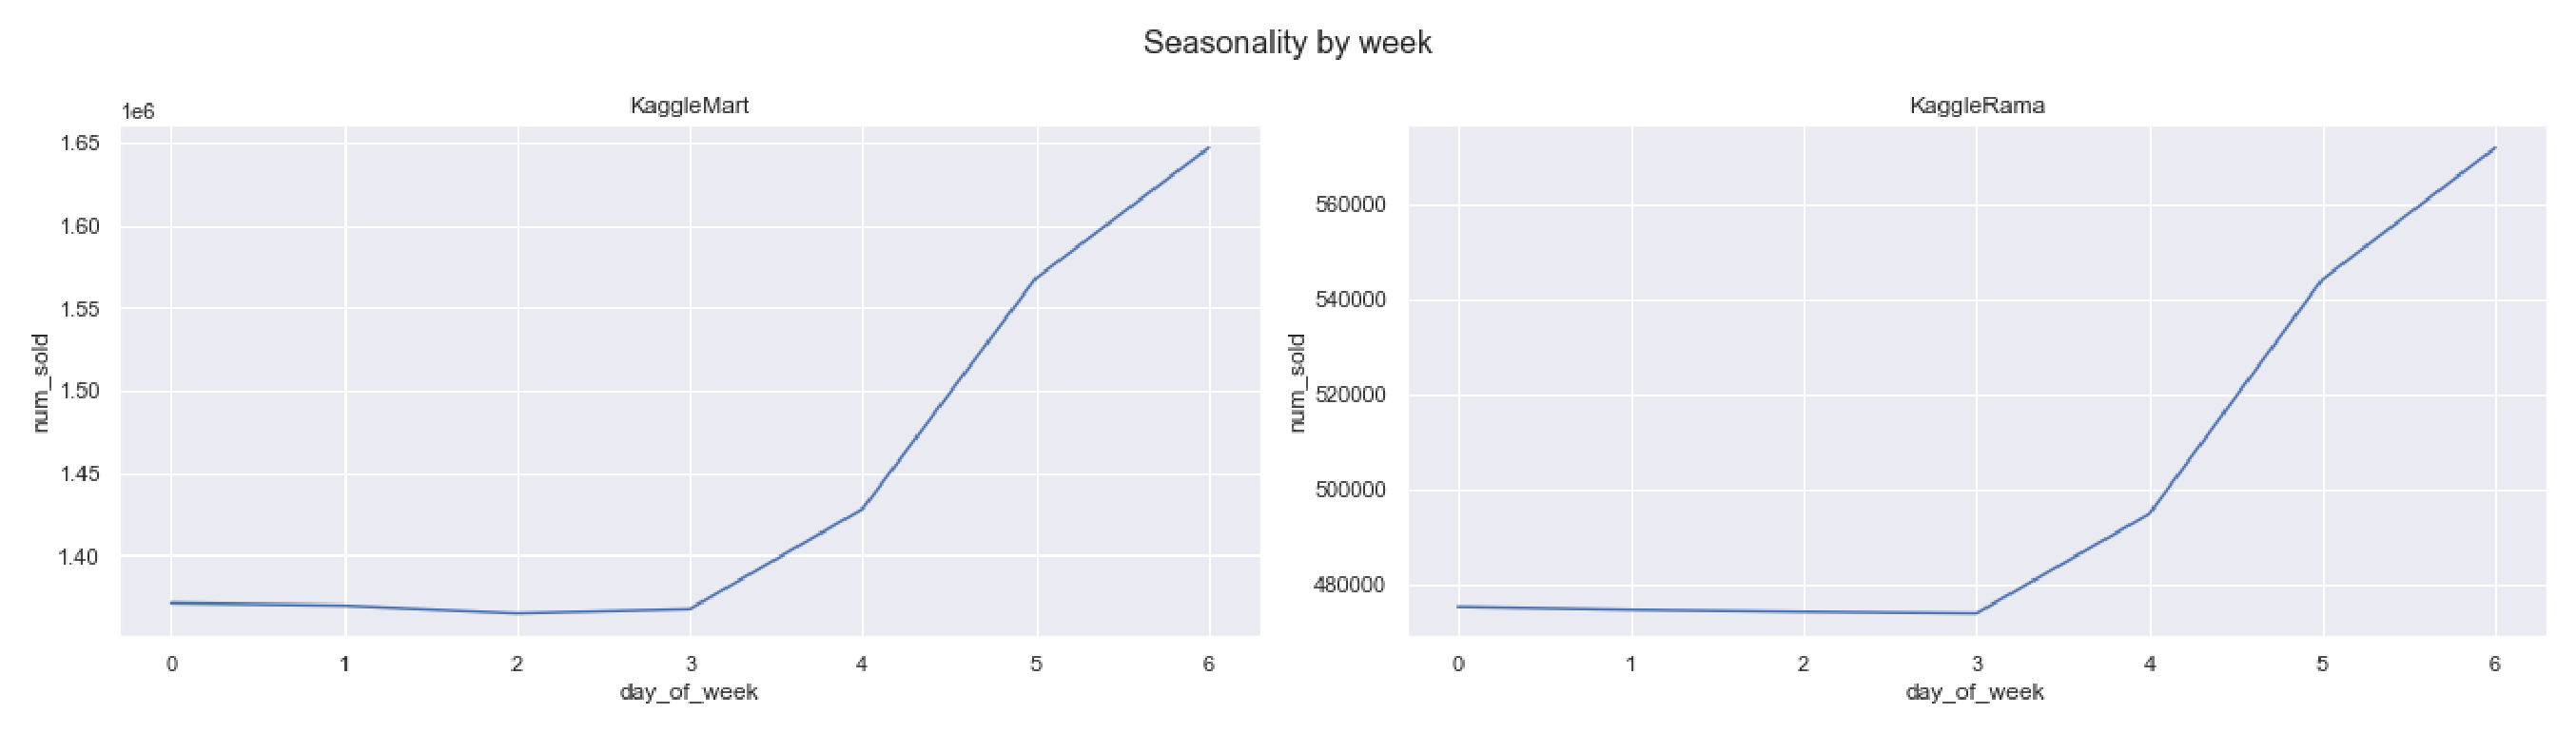
\includegraphics[scale=0.25]{week-feature.eps}
%DIFDELCMD < 	%%%
%DIF <   \includegraphics[width=0.5\textwidth]{figures//OutAspect_target.eps}\\
	%DIFDELCMD < \caption{%
{%DIFAUXCMD
\DIFdelFL{weekday feature}}%DIFAUXCMD
%DIFDELCMD < \label{fig:OutAspect-target}
%DIFDELCMD < \end{figure}
%DIFDELCMD < %%%
\DIFdel{At the same time, 
in order to make Fourier transform understand the monthly data, we remove the sine value and cosine value of the month.At the same time, we also considered the feature of important festivals in the year. 
Finally, 
we get that the features of the training set include 23 features.
}\DIFdelend \DIFaddbegin \begin{equation}\DIFadd{\label{eq:test}
a = b \times \sqrt{ab}
}\end{equation}
\DIFaddend 

\DIFdelbegin \section{\DIFdel{Model Train}} %DIFAUXCMD
\addtocounter{section}{-1}%DIFAUXCMD
%DIFDELCMD < \label{sec-experiment}
%DIFDELCMD < %%%
\DIFdel{We use Ridge regression from the "linear_model" module to correlate the relationship betweensales and time features , and predict on the test set.Train the model with time features as X and sales as y.The sales of the test set is predicted according to the time features of the test set. Finally, we obtained the total sales prediction curve.}\DIFdelend \DIFaddbegin \blindmathpaper
\DIFaddend 

\DIFdelbegin %DIFDELCMD < \begin{figure}[H]
%DIFDELCMD < 	\centering
%DIFDELCMD < 	\selectcolormodel{rgb}
%DIFDELCMD < 	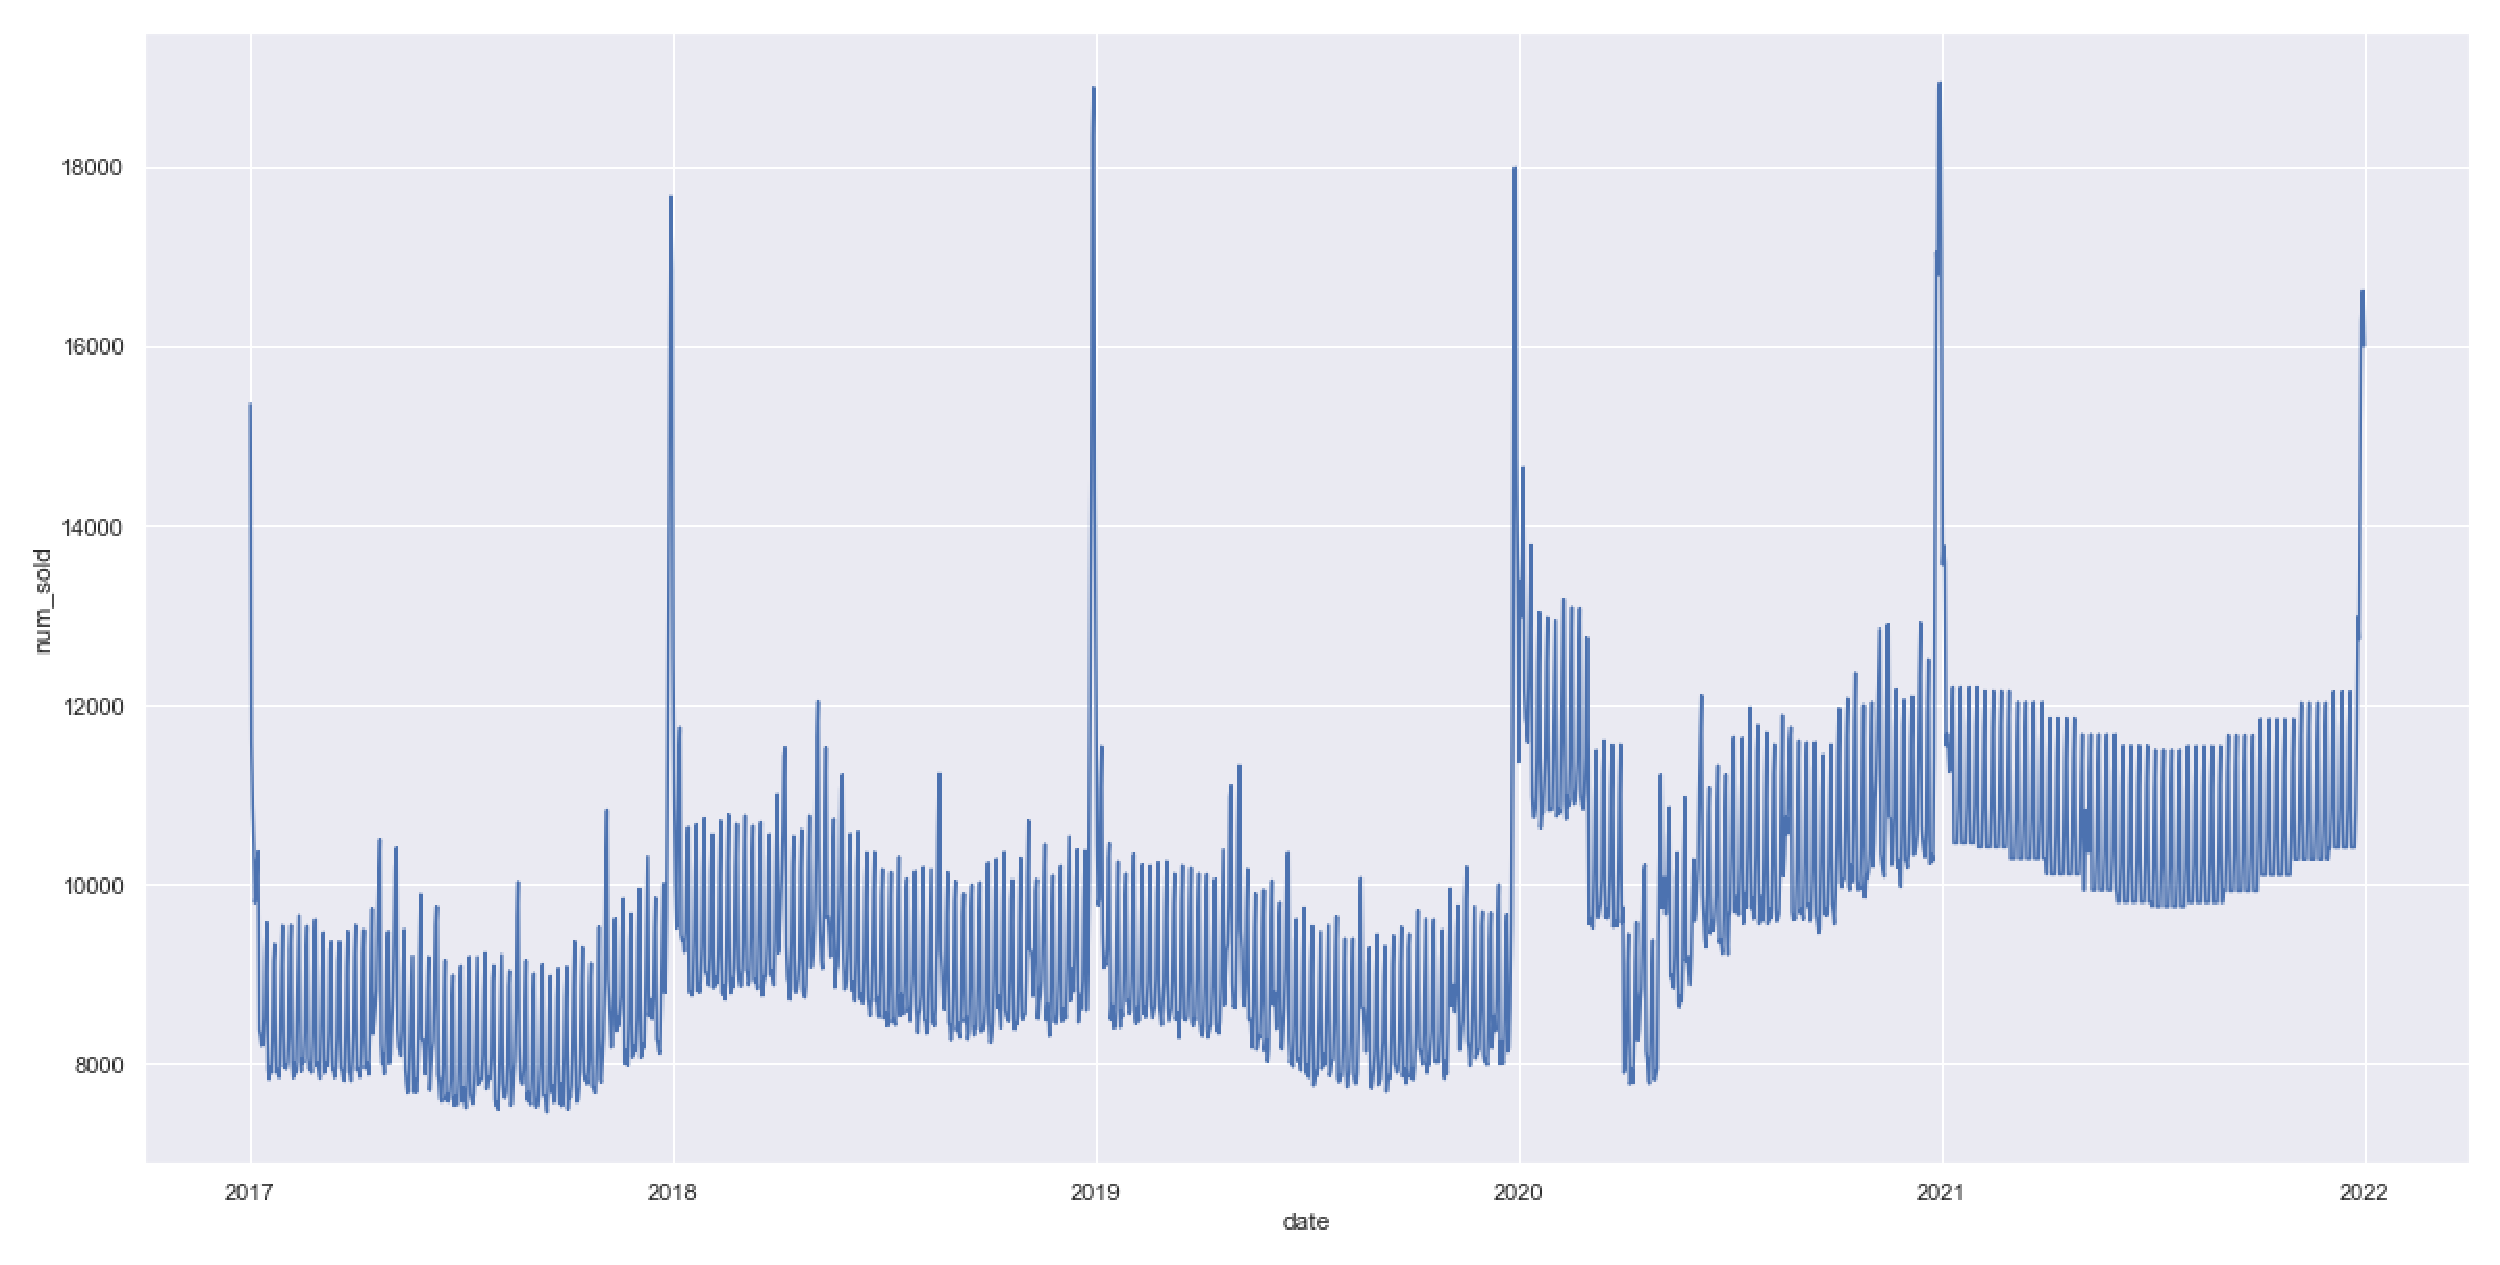
\includegraphics[scale=0.3]{total-sales.eps}
%DIFDELCMD < 	%%%
%DIF <   \includegraphics[width=0.5\textwidth]{figures//OutAspect_target.eps}\\
	%DIFDELCMD < \caption{%
{%DIFAUXCMD
\DIFdelFL{total sales forecasting}}%DIFAUXCMD
%DIFDELCMD < \label{fig:OutAspect-target}
%DIFDELCMD < \end{figure}
%DIFDELCMD < %%%
\DIFdelend \DIFaddbegin \section{\DIFadd{Preliminaries}} \label{sec-preliminaries}
\DIFaddend 

\DIFdelbegin \DIFdel{We found that the proportion of sales for a product has a cyclical variation with a period of two years. Therefore, we assign the daily proportion of sales for each product in 2019 to 2021.
}\DIFdelend \DIFaddbegin \blindtext
\DIFaddend 

\DIFdelbegin %DIFDELCMD < \begin{figure}[htb]
%DIFDELCMD < 	\centering
%DIFDELCMD < 	\selectcolormodel{rgb}
%DIFDELCMD < 	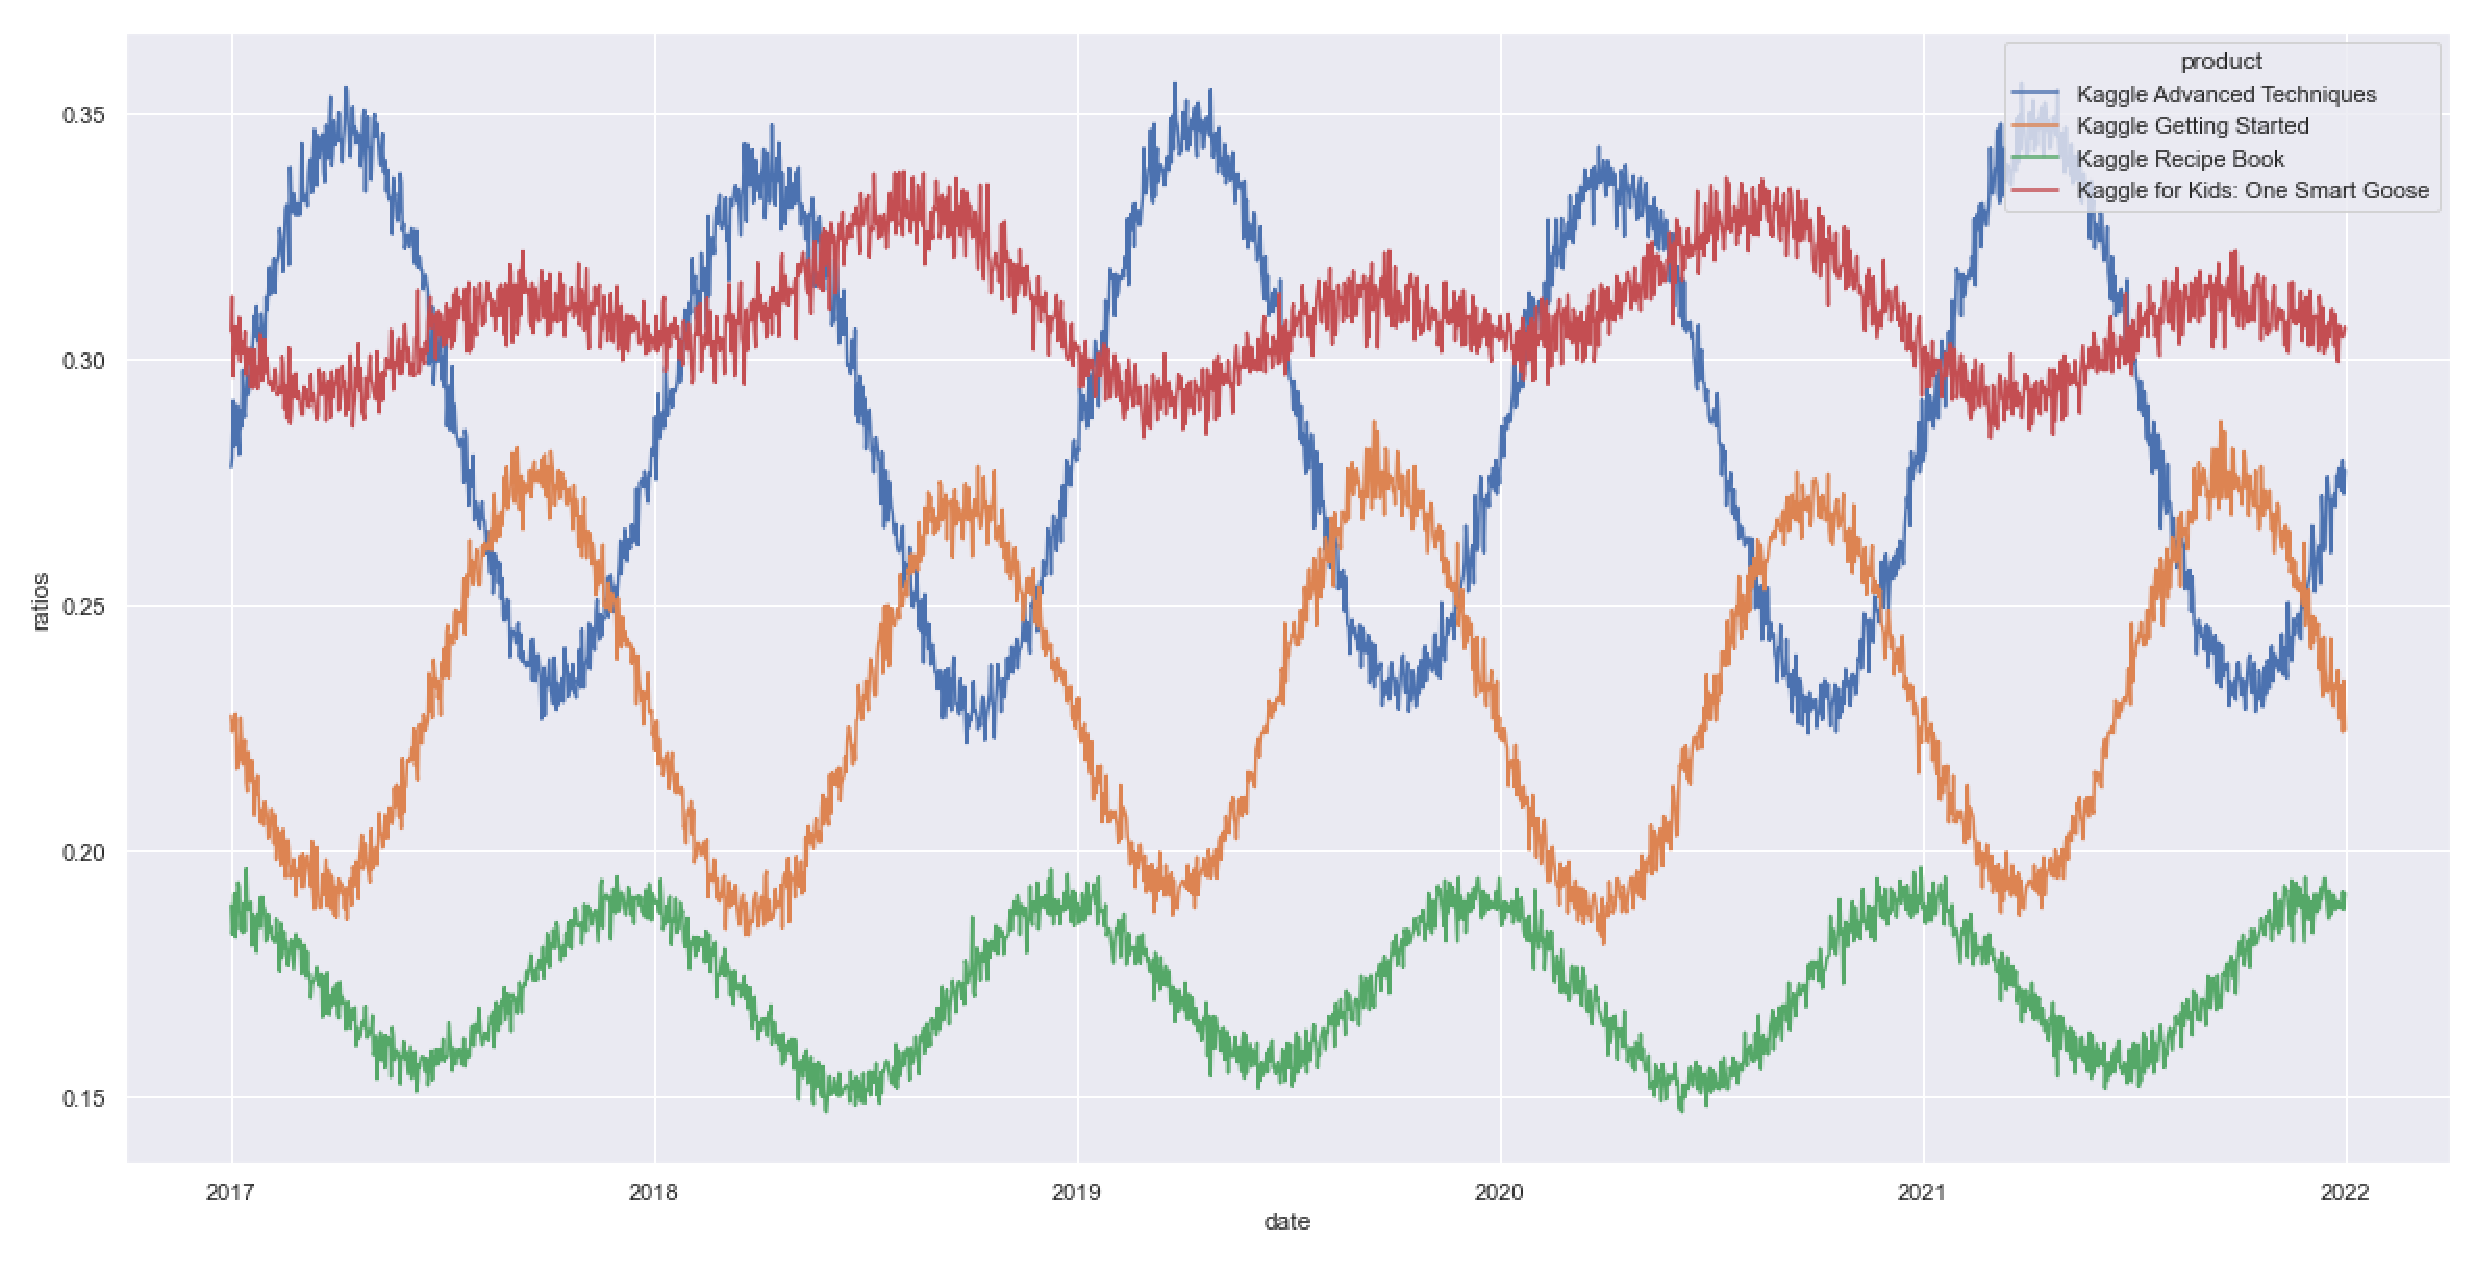
\includegraphics[scale=0.3]{product-ratio-for.eps}
%DIFDELCMD < 	%%%
%DIF <   \includegraphics[width=0.5\textwidth]{figures//OutAspect_target.eps}\\
	%DIFDELCMD < \caption{%
{%DIFAUXCMD
\DIFdelFL{Product Ratio Forecast}}%DIFAUXCMD
%DIFDELCMD < \label{fig:OutAspect-target}
%DIFDELCMD < \end{figure}
%DIFDELCMD < %%%
\DIFdelend \DIFaddbegin \gliMarker  %DIF > TODO: GLi Here
\DIFaddend 


\DIFdelbegin \DIFdel{We assume that the proportion of sales in countries in 2021 is the same as in 2020. In 2020, the proportion of sales in countries accounts for1/6.The proportion of different stores remains fixed, 
KaggleMart accounts for75\%,
and KaggleRama accounts for 25\%.
}\DIFdelend \DIFaddbegin \section{\DIFadd{Method}} \label{sec-method}
\DIFaddend 

\DIFdelbegin %DIFDELCMD < \begin{figure}[H]
%DIFDELCMD < 	%%%
\DIFdelendFL \DIFaddbeginFL \blindtext
\blindlist{itemize}[3]
\blinditemize
\blindenumerate

\blindmathtrue
\blindmathfalse
\blinddescription

\qwuMarker %DIF > TODO: QWu Here

\section{\DIFaddFL{Experiment and Analysis}} \label{sec-experiment}


\begin{table}  \DIFaddendFL \centering
  \DIFdelbeginFL %DIFDELCMD < \selectcolormodel{rgb}
%DIFDELCMD < 	\includegraphics[scale=0.2]{final-for.eps}
%DIFDELCMD < 	%%%
%DIF <   \includegraphics[width=0.5\textwidth]{figures//OutAspect_target.eps}\\
	\DIFdelendFL \caption{\DIFdelbeginFL \DIFdelFL{Final Forecasting}\DIFdelendFL \DIFaddbeginFL \DIFaddFL{Precision Comparison on Event Detection Methods}\DIFaddendFL }
  \DIFdelbeginFL %DIFDELCMD < \label{fig:OutAspect-target}
%DIFDELCMD < \end{figure}
%DIFDELCMD < %%%
\DIFdelend \DIFaddbegin \label{tbl:overall-experiments}
  \begin{tabular}{cccc}
\toprule
    %DIF >  after \\: \hline or \cline{col1-col2} \cline{col3-col4} ...
    & \DIFadd{OR Event Detection }& \DIFadd{AC Event Detection }& \DIFadd{TC Event Detection }\\
\midrule
    \DIFadd{precision }& \DIFadd{0.83 }& \DIFadd{0.69 }& \DIFadd{0.46 }\\
    \DIFadd{recall }& \DIFadd{0.68 }& \DIFadd{0.48 }& \DIFadd{0.36 }\\
    \DIFadd{F-score }& \DIFadd{0.747 }& \DIFadd{0.57 }& \DIFadd{0.4 }\\
\bottomrule
\end{tabular}
\end{table}
\DIFaddend 


\section{Conclusions} \label{sec-conclusions}
\DIFdelbegin \DIFdel{This is a time series forecasting problem that includes complex elements.Simplifying the effects of complex factors through analyzing patterns discovered through single factor analysis.Use linear regression method to predict the relationship between sales volume and time characteristics.
}\DIFdelend \DIFaddbegin 

\DIFaddend \blindtext
\DIFaddbegin 

\section*{\DIFadd{Acknowledgement}}

\lipsum[1]


\DIFadd{The authors would like to thank \ldots
}\DIFaddend 

